% !TEX root = ../main.tex



\bigskip
\chapter{Vigra Graph Library} \label{ch:vigra_graph_lib}

Vigra \cite{software_vigra} is library for image processing and analysis.
Vigra provides customizable and genric algorithms and datastructures.
Vigra is capable of dealing with multi-dimensional images 
and many algorithms are implemented for arbitrary data types
and dimensions.
Vigra has a wide range of features from simple convolution filters, 
tensor based image processing to machine learning algorithms 
as decision trees.

To simplify the implementation of algorithms for images arbitrary 
dimension, vigra uses a grid graph which is capable of
dealing with any dimension.

Within this thesis we extend the concept graph based image processing
within vigra w.r.t. graphs of any structure.
We put main emphasis on extendability while keeping the usage very simple.


\section{Graph API's}\label{sec:graph_apis}

We strongly belief is is beneficial to use an existing API's for
graphs instead of inventing an own graph API for Vigra.
Coming up with a new API is not straight forward
since one might to think of any future use case this API.
In addition, users became accustomed with existing API's as 
the LEMON or Boost graph API.
Existing algorithms of a particular API can be reused if we stick
to that API.




\subsection{LEMON Graph API's}\label{sec:lemon_graph_apis}
    LEMON \citet{ software_lemon} 
    stand for  ``Library for Efficient Modeling and Optimization in Networks.''.
    It is an open source C++ library with algorithms and data structures 
    related to directed and undirected graphs.
    The extensive usage of templates make this library very flexible.
    While lemon provides a huge set of graph algorithms,
    we are mostly interested in the graph API itself.
    In the following we will give a brief overview of lemons graph 
    API and the related concepts.
    Explaining the complete lemon graph API in detail
    is beyond the scope of this thesis.
    Interested readers are referred to \citet{software_lemon}.
    We will only discuss the API for undirected graphs since any
    graph algorithm we implemented within this thesis
    will work on undirected graphs.

\subsubsection{Graph Items}
    Any undirected graph class fulfilling the lemon API needs to define 
    the following \emph{descriptor} types to represent the graph items.
    \begin{compactitem}
    \item \lstinline{Graph::Edge}
    \item \lstinline{Graph::Arc}
    \item \lstinline{Graph::Node}
    \end{compactitem}
    These \emph{descriptor} should be cheap types which can be copied
    and passed with almost no overhead.
    In addition, descriptor has an unique id
    \footnote{ unique id w.r.t. the item type. 
    Therefore  multiple  nodes cannot have the same id.
    The same holds line for edges and arcs.
    But there might be a node and edge which have the same id}.
    These id's can be accessed via \lstinline{Graph::id(Node)}, \lstinline{Graph::id(Edge)} and \lstinline{Graph::id(Arc)}.
    These id's can not only be dense but also sparse, which is very
    important for an efficient handling of grid graph edge ids.



\subsubsection{Iterators}

    Within lemon a very convenient mechanism is used to iterate over
    nodes, edges and arcs.
    A special constant \lstinline{INVALID} is used to determine if 
    an iterator reached the end.

    \begin{minipage}{\textwidth}\vspace{-0.75cm}\begin{lstlisting}[language=c++]
    // iterate over nodes
    for(Graph::NodeIt v(g); v!= lemon::INVALID; ++v){/*...*/}

    // iterate over edges
    for(Graph::EdgeIt e(g); e!= lemon::INVALID; ++e){/*...*/}

    // iterate over arcs
    for(Graph::ArcIt a(g); a!= lemon::INVALID; ++a){/*...*/}

    // use arcs to iterate over neighbor nodes
    for(Graph::OutArcIt a(g,n); a!= lemon::INVALID; ++a){
        const Node neighborNode = g.target(a);
        /*...*/
    }
    \end{lstlisting}\end{minipage}\vspace{0.5cm}

    Any iterator is convertible to the corresponding item which
    is iterated without using \lstinline{operator*()}.

\subsubsection{Map Concept}

    In lemon, graph classes store only the structure of the graph itself.
    All addition data for nodes, edges and arcs is stored 
    in \emph{maps}. 
    Any graph has default implementations for graph maps which
    can be accessed in the following way.

    \begin{minipage}{\textwidth}\vspace{-0.75cm}\begin{lstlisting}[language=c++]
    // edge map (for data as edge weights)
    Graph::EdgeMap<float> edgeMap(g); 

    // read and write data 
    for(Graph::EdgeIt e(g); e!= lemon::INVALID; ++e){
        // read
        const float val = edgeMap[*e];
        // write
        edgeMap[*e] = std::exp(-1.0*a);
    }

    // node map (for node related data as node labelings )
    Graph::NodeMap<usigned int> nodeMap(g);
    for(Graph::NodeIt v(g); v!= lemon::INVALID; ++v){
        // read
        const unsigned int val = nodeMap[*e];
        // write
        nodeMap[*e] = val+1;
    }
    \end{lstlisting}\end{minipage}\vspace{0.5cm}


    Custom maps can be implemented very easy:

    \begin{minipage}{\textwidth}\vspace{-0.75cm}\begin{lstlisting}[language=c++]
    template<class Graph>
    class ImplicitEdgeMap {
    public:
        typedef typename Graph::Edge Key;
        typedef double Value;
        Value operator[](Key edge) const { 
            Value a;
            /*...*/
            return a;
        }
    };
    \end{lstlisting}\end{minipage}\vspace{0.5cm}

\subsection{BOOST Graph API's}\label{sec:boost_graph_apis}
Give brief overview of boost graph api





\subsection{VIGRA Graph API}
Explain why which api is used and how it is extended



\section{Implementation}\label{sec:vigra_graph_lib_impl}

The most important concept for graph based image processing
is the \emph{region adjacency graph} (RAG) (see \cref{fig:make_rag}).

A RAG is extracted from a labeled \emph{base graph}.
In the first step of graph based image processing, the base 
graph is usually a grid graph, and the labeling is a label image
as in \cref{fig:make_rag} .
To encode a RAG we need a undirected graph, 
and a mapping from the base graphs edges and nodes to the RAG 
needs to be stored.

The implementation of grid graphs is explained in \cref{sec:graphs_grid_graph}, 
a basic undirected graphs implementation will be discussed in \cref{sec:graphs_adjacency_list_graph}.
The implementation details of the \emph{region adjacency graph} concept will 
be given in  \cref{sec:graphs_rag}.

For hierarchical clustering we provide a specialized graph, named \emph{merge graph}.


To implemented structured clustering algorithms (see \cref{sec:rw_hc} we
need a graph which supports the contraction of edges.
Also a mechanism to merge node and edge features is needed.
Within \cref{sec:graphs_merge_graph} we propose  a very flexible
and concept for hierarchical clustering based on a specialized graph,
called \emph{merge graph}.


A generic set of algorithms which work on any graph
implemented within the VIGRA graph api is presented 
in \cref{sec:graph_graph_algorithms}.

While the core implementation of any algorithm is in C++
VIGRA provides python binding to make almost
any algorithm available in Python.
To provide a generic Python interface for any proposed
graph, we need to introduce a few concepts 
to make the python wrapped graph API very \emph{Pythonic}


\section{Graphs}


\subsection{Grid Graph} \label{sec:graphs_grid_graph}

\missingfigure{show grid graph here}

    \lstinline{vigra::GridGraph<DIM,DIRECTED_TAG>}

\subsection{Adjacency List Graph} \label{sec:graphs_adjacency_list_graph}


    \begin{minipage}{\textwidth}\vspace{-0.75cm}\begin{lstlisting}[language=c++]
    typedef AdjacencyListGraph Graph;

    // construct graph
    Graph g;

    // add nodes (id will be asigned automatically)
    Graph::Node n0 = g.addNode() 

    // add node with an explicit id
    Graph::Node n3 = g.addNode(3)

    // add edges from existing nodes
    Graph::Edge e0 = g.addEdge(n0,n1)

    // add edges and nodes simultaneous 
    Graph::Edge e1 = g.addEdge(2,3)

    // no parallel edges 
    Graph::Edge e2 = g.addEdge(2,3)
    assert(e1==e2)  
    \end{lstlisting}\end{minipage}\vspace{0.5cm}



\subsection{Region Adjacency Graph} \label{sec:graphs_rag}


\subsection{Merge Graph} \label{sec:graphs_merge_graph}
To implemented structured clustering algorithms (see \cref{???}) we
need a graph which supports the contraction of edges.
Also a mechanism to merge node and edge features is needed.
Experiments suggest that the edge contraction is more expensive
than feature merging an can even be a bottleneck for huge 3D data 
(see \cref{???} ).
Therefore it is crucial to implemented the MergeGraph (MG) very carefully.
\begin{figure}
    \centering
    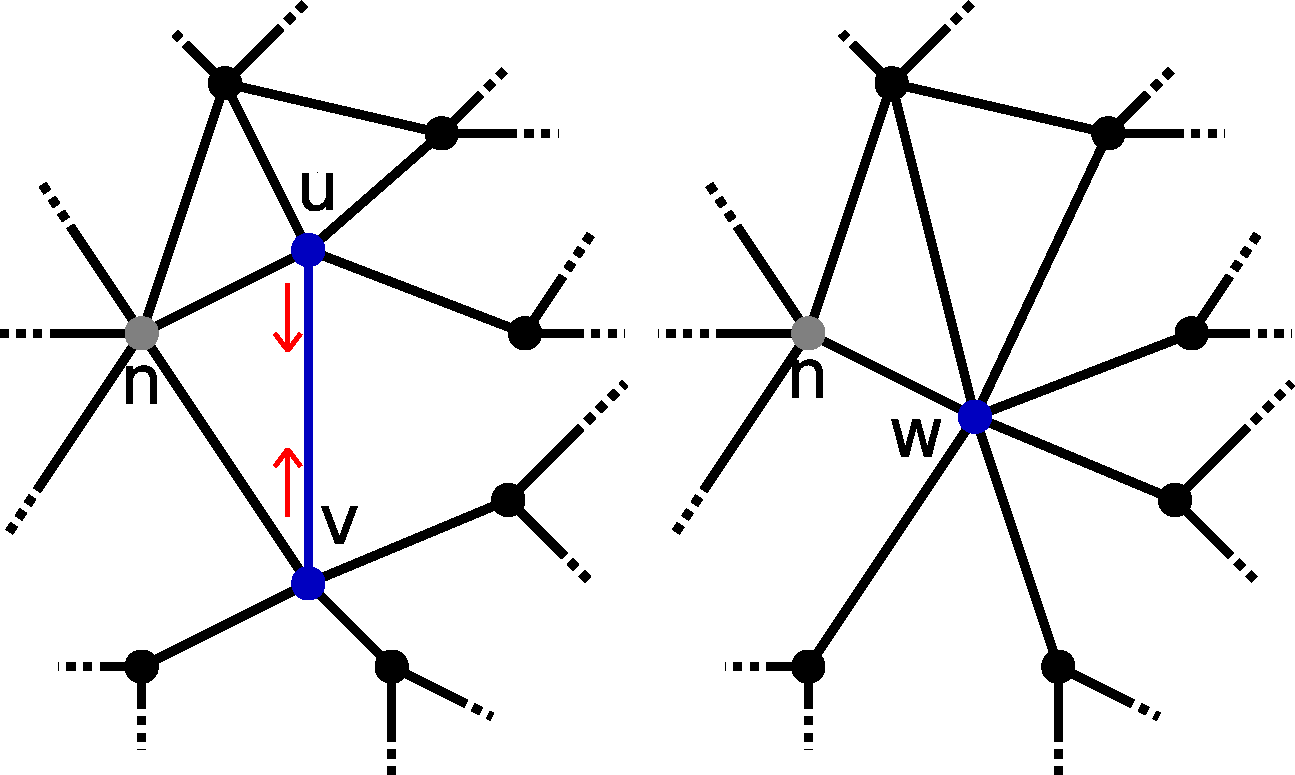
\includegraphics[width=0.35\textwidth]{fig/contraction.pdf}

    \addtocontents{lof}{%
        \vspace{1cm}
        \protect\centerline{%
            \protect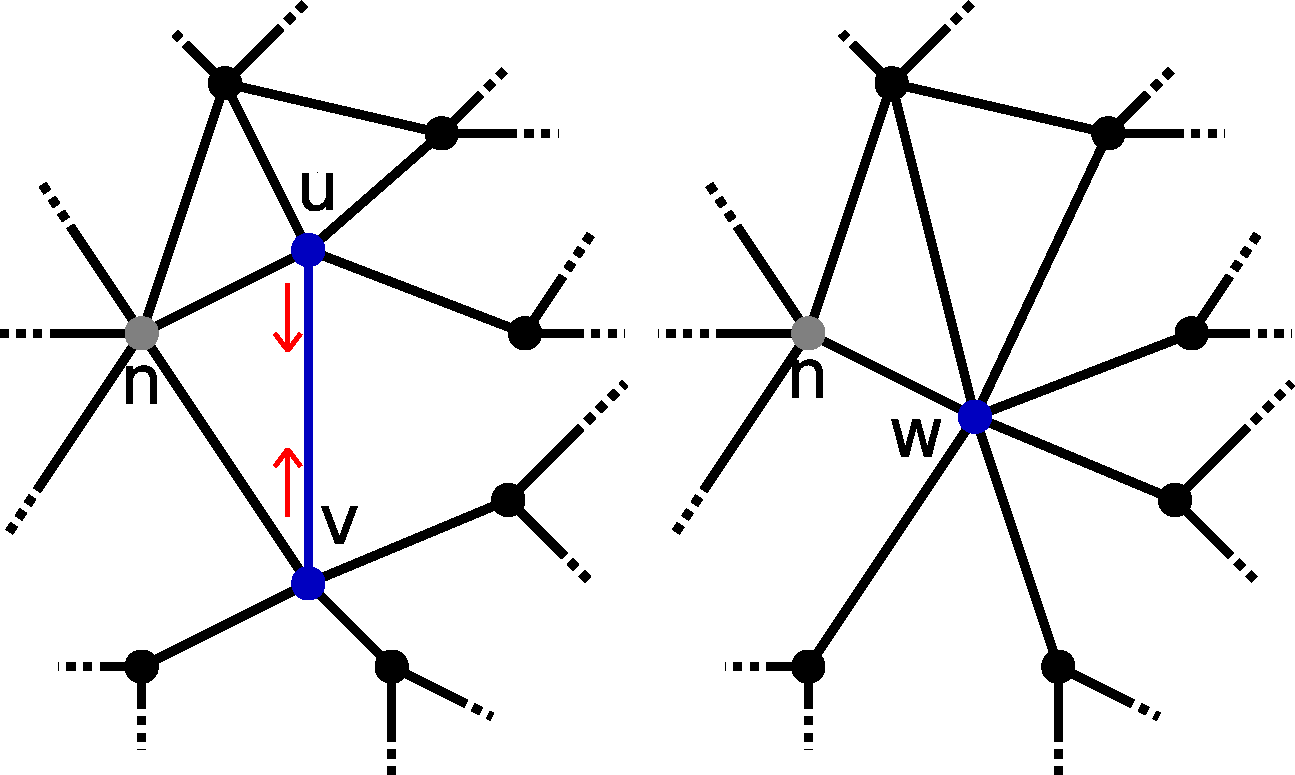
\includegraphics[width=.075\linewidth]{fig/contraction.pdf} 
        }%
    }%

    \caption[Schematic edge contraction]{ Schematic edge contraction: Node $u$ and $v$ is merged into node $w$.
        Note the gray node $n$ which is connected to $u$ and $v$.
        After the contraction, edges $\{ n,u\}$ and $\{ n,v\}$ are also merged into 
        a single edge $\{ n, w\}$ 
    }
    \label{fig:figlabel}
\end{figure}


   

\begin{center}
    \begin{tikzpicture}
        \umlclass[template=Graph]{MergeGraphAdpator}
        {
            \\// union find data structures                     \\
            - edgeUfd               : IterablePartiton          \\
            - nodeUfd               : IterablePartiton          \\ 
            - nodesAdjacency        : AdjacencySetVector        \\

            \\// callbacks                                      \\
            - mergeNodeCallBacks    : MergeNodeCallBackVector   \\
            - mergeEdgeCallBack     : MergeEdgeCallBackVector   \\
            - eraseEdgeCallBack     : EraseEdgeCallBackVector   \\
        }
        {
            \\// LEMON API for undirected graphs                \\
                $\ldots$                                        \\
            \\// register callbacks                             \\ 
            + registerMergeNodeCallBack(f : MergeNodeCallBack)  \\
            + registerMergeEdgeCallBack(f : MergeEdgeCallBack)  \\
            + registerEraseEdgeCallBack(f : EraseEdgeCallBack)  \\

            \\// modify graph                                   \\
            + contractEdge(edge : Edge)     : Node              \\

            \\// find representatives                           \\
            + reprNode(node : Node)         : Node              \\
            + reprEdge(edge : Edge)         : Edge              \\ 

            \\// get base graph                                 \\
            + graph()                       : Graph             \\
        } 
    \end{tikzpicture}
\end{center}



\begin{center}
    \begin{tikzpicture}
        \umlclass[template=MergeGraph]{ClusterOperatorInterface}
        {

        }
        {
            \\// contract next edge and get weight              \\
            + contractionEdge(edge : Edge)         : Edge       \\ 
            + contractionWeight(edge : Edge)       : Edge       \\
            \\// get base graph                                 \\
            + mergeGraph()                  : MergeGraph        \\
        } 
    \end{tikzpicture}
\end{center}


\begin{center}
    \begin{tikzpicture}
        \umlclass[template=ClusterOperator]{HierarchicalClustering}
        {

        }
        {
            + cluster()                     : void        \\
            + reprLabels(nodeMap : NodeMap) : void        \\      
        } 
    \end{tikzpicture}
\end{center}


   We propose and implemented the following design:
   \begin{compactitem}
       \item  A base graph is attached to a merge graph  and  a merge graph will
            always ``view'' to
       \item  Union find data structure for nodes
       \item  Union find data structure for edges
   \end{compactitem}



   \lstinline{vigra::MergeGraphAdaptor<DIM,DIRECTED_TAG>}

\subsection{Region Adjacency Graph}

    \missingfigure{show region adjacency graph here}

\section{Graph Algorithms} \label{sec:graph_graph_algorithms}

    \subsection{Multicut}

    \subsection{Hierarchical Clustering}

    \subsection{Mst Algorithms}

    \subsection{Watershed Algorithms}

    \subsection{Smoothing Algorithms}





\section{Python}




\begin{flushright}{\slshape    
(1) Beautiful is better than ugly. \\ \label{cit:line_a}
(2) Explicit is better than implicit. \\ \label{cit:line_b}
(3) Simple is better than complex. \\
(4) Complex is better than complicated. \\
(5) Flat is better than nested. \\
(6) Sparse is better than dense. \\
(7) Readability counts. \\
(8) Special cases aren't special enough to break the rules. \\
(9) Although practicality beats purity. \\
(10) Errors should never pass silently. \\
(11) Unless explicitly silenced. \\
(12) In the face of ambiguity, refuse the temptation to guess. \\
(13) There should be one-- and preferably only one --obvious way to do it. \\
(14) Although that way may not be obvious at first unless you're Dutch. \\
(15) Now is better than never. \\
(16) Although never is often better than *right* now. \\
(17) If the implementation is hard to explain, it's a bad idea. \\
(18) If the implementation is easy to explain, it may be a good idea. \\
(19) Namespaces are one honking great idea -- let's do more of those! } \\ \medskip
--- The Zen of Python
\end{flushright}
\captionof{figure}{ 
    The Zen of Python
}\label{fig:zen_of_python}



Since \cref{fig:zen_of_python}(2)-(3)


On the python side, we want node-maps,edge-maps and arc-maps to be stored 
as numpy arrays for ??? reasons.:
\begin{compactitem}
    \item Numpy arrays are the standard for storing multidimensional data in python.
    The fast C implementations and a vectorized API of numpy make it very easy to write 
    fast python code within a few lines.
    Virtually any python user will be familiar with the numpy API and therefore it 
    seems to be natural to store graph maps within numpy arrays.
    \item Vigra provides an mechanism to pass numpy arrays to C++.
    Therefore no new mechanism needs to be implemented to transfer graph
    maps from python to C++.
    This will not only simplify writing extension for the new vigra graph api,
    but also it will reduce the glue code since we can use well tested existing
    solutions.
    \item New algorithms might be implemented in pure python with a mix of
    existing numpy functions and new functions provided within vigras graph api.
    As a proof of concept we implemented ??? in pure python with vigras
    fresh graph api in \cref{???}.
\end{compactitem}

On the C++ side, numpy arrays are stored in MultiArrayViews.
Since API of MultiArrayViews \cite{software_vigra_multiarray_api} does
not implemented the API  of LEMON graph maps (e.g. node-maps,edge-maps and arc-maps).
 

\begin{lstlisting}[language=python]
vigra.graphs.foobar(graph,nodeFeatures)
\end{lstlisting}
\section{Some Tikz stuff}




\begin{lstlisting}[language=c++]
static NumpyAnyArray ConverterStruct::foobar(
    const Graph & graph , 
    const typename PyNodeMapTraits<Graph, UInt32>::Array & nodeArray
){
    typename PyNodeMapTraits<Graph, UInt32>::Map nodeArrayMap(graph,nodeArray)

    // code using LEMON Map Api 
}
\end{lstlisting}
